\section{Transient solver} \label{sec:transient_solver}

The full transient equations are more difficult to solve than the steady state problem as the resistance term in the momentum is now time dependent and we must retain all the terms in the discrete continuity equation \eqref{discrete_continuity_eqn}. The equations must be stepped forward in time using a scheme which is both accurate and numerically stable. 

\subsection{Theta method}

The $\theta$-method is a generalisation of the Crank-Nicolson method which allows the scheme to be made more or less implicit. In general the scheme takes the form
\begin{align}
\frac{u_i^{n+1} - u_i^{n}}{\Delta t} = \theta F_i^{n+1}\left(u,x,t,\pardiv{}{u}{x},\ldots \right) + (1-\theta) F_i^{n}\left(u,x,t,\pardiv{}{u}{x},\ldots \right),
\end{align}
where $\theta \in [0,1]$. If $\theta = 0$ then the scheme is the explicit forward Euler method, if $\theta = 1$ then it is the fully implicit backward Euler method and if $\theta = 1/2$ then it is the Crank-Nicolson method. Usually the Crank-Nicolson scheme is preferred to both the forward and backward Euler methods as it is second order accurate whereas they are both only first order accurate. However the approximate solutions found using the Crank-Nicolson scheme sometimes include spurious oscillations so it may be preferable to use the less accurate implicit scheme in certain situations.


Using the $\theta$-method on the continuity equation \eqref{discrete_continuity_eqn} we have
\begin{align}
\mathbf{K}^T \left( \theta \mathbf{Q}^{n+1} + (1-\theta)\mathbf{Q}^{n} \right) + \mathbf{D} \left( \frac{\mathbf{H}^{n+1} - \mathbf{H}^{n}}{\Delta t} \right) = \mathbf{C}.
\end{align}
Then for the momentum equation \eqref{discrete_momentum_eqn} we have
\begin{align}
\frac{\mathbf{Q}^{n+1} - \mathbf{Q}^{n}}{\Delta t} = \mathbf{R}\left( \theta \mathbf{Q}^{n+1} + (1-\theta)\mathbf{Q}^{n}, \theta \mathbf{K} \mathbf{H}^{n+1} + (1-\theta) \mathbf{K} \mathbf{H}^n \right).
\end{align}
At time-step $n$ the pipe flow rates $\mathbf{Q}^{n}$ and nodal heads $\mathbf{H}^{n}$ are known and we would like to estimate the solution at the subsequent time-step $n+1$. The steady state solution $\mathbf{Q}^{0}$ and $\mathbf{H}^{0}$ is used to initialise the scheme.

\subsubsection{Newton iteration} 

Since the solution is known at time-step $n$ only the solution at time-step $n+1$ needs to be split into a known/guessed part and a correction i.e. $\mathbf{Q}^{n+1} = \mathbf{Q}^{n+1,g} + \mathbf{Q}^{n+1,c}$ and $\mathbf{H}^{n+1} = \mathbf{H}^{n+1,g} + \mathbf{H}^{n+1,c}$. The resitance term is then approximated as
\begin{align*}
\mathbf{R}(\mathbf{Q}, \mathbf{K} \mathbf{H}) \approx \mathbf{R}\left(\bar{\mathbf{Q}}, \mathbf{K} \bar{\mathbf{H}} \right) + \pardiv{}{\mathbf{R}}{\mathbf{Q}} \Bigg\vert_{\bar{\mathbf{Q}}} \theta \mathbf{Q}^{n+1,c} + \pardiv{}{\mathbf{R}}{\mathbf{K} \mathbf{H}} \Bigg\vert_{\mathbf{K} \bar{\mathbf{H}}} \theta \mathbf{K} \mathbf{H}^{n+1,c},
\end{align*}
where $\bar{\mathbf{Q}}=\theta \mathbf{Q}^{n+1,g} + (1-\theta) \mathbf{Q}^{n}$, $\bar{\mathbf{H}}=\theta \mathbf{H}^{n+1,g} + (1-\theta) \mathbf{H}^{n}$. Splitting into a known part and correction at the next time step the continuity equation is given by
\begin{align}\label{discrete_transient_continuity_eqn_newton}
\theta \mathbf{K}^T \mathbf{Q}^{n+1,c} + \frac{1}{\Delta t} \mathbf{D} \mathbf{H}^{n+1,c} = \mathbf{C} - \mathbf{K}^T \bar{\mathbf{Q}} - \frac{1}{\Delta t} \mathbf{D} \left( \mathbf{H}^{n+1,g} - \mathbf{H}^{n} \right),
\end{align}
and the momentum equation is given by
\begin{align}\label{discrete_transient_momentum_eqn_newton}
\left(\frac{1}{\Delta t} \mathbf{I} - \theta \pardiv{}{\mathbf{R}}{\mathbf{Q}} \Bigg\vert_{\bar{\mathbf{Q}}} \right) \mathbf{Q}^{n+1,c} - \theta \pardiv{}{\mathbf{R}}{\mathbf{K} \mathbf{H}} \Bigg\vert_{\mathbf{K} \bar{\mathbf{H}}} \mathbf{K} \mathbf{H}^{n+1,c} = \mathbf{R}\left(\bar{\mathbf{Q}}, \mathbf{K} \bar{\mathbf{H}} \right) - \frac{1}{\Delta t} \left(\mathbf{Q}^{n+1,g} - \mathbf{Q}^{n} \right).
\end{align} 
Equations \eqref{discrete_transient_continuity_eqn_newton} and \eqref{discrete_transient_momentum_eqn_newton} must be solved together as the single system of equations
\begin{align}\label{discrete_transient_system}
\begin{bmatrix}
\theta \mathbf{K}^T & \frac{1}{\Delta t}\mathbf{D} \\
\frac{1}{\Delta t}\mathbf{I}-\theta \bar{\mathbf{J}} & - \theta \bar{\mathbf{G}}
\end{bmatrix} 
\begin{bmatrix}
\mathbf{Q}^{n+1,c} \\ \mathbf{H}^{n+1,c}
\end{bmatrix} = \begin{bmatrix}
\mathbf{C} - \mathbf{K}^T \bar{\mathbf{Q}} - \frac{1}{\Delta t} \mathbf{D} \left( \mathbf{H}^{n+1,g} - \mathbf{H}^{n} \right) \\
\mathbf{R}\left(\bar{\mathbf{Q}}, \mathbf{K} \bar{\mathbf{H}} \right) - \frac{1}{\Delta t} \left(\mathbf{Q}^{n+1,g} - \mathbf{Q}^{n} \right)
\end{bmatrix},
\end{align}
where $\bar{\mathbf{J}} = \pardiv{}{\mathbf{R}}{\mathbf{Q}} \big\vert_{\bar{\mathbf{Q}}}$ and $\bar{\mathbf{G}} = \pardiv{}{\mathbf{R}}{\mathbf{K} \mathbf{H}} \big\vert_{\mathbf{K} \bar{\mathbf{H}}} \mathbf{K} $. In a similar manner to the steady solver the system of equations \eqref{discrete_transient_system} would be solved for the corrections, $\mathbf{Q}^{n+1,c}$ and $\mathbf{H}^{n+1,c}$, these would then be used to update the guess $\mathbf{Q}^{n+1,g} \rightarrow \mathbf{Q}^{n+1,g} + \mathbf{Q}^{n+1,c} $ and $\mathbf{H}^{n+1,g} \rightarrow \mathbf{H}^{n+1,g} + \mathbf{H}^{n+1,c} $ and then the process would be repeated until the corrections are sufficiently small. After updating the simulation time $t \rightarrow t + \Delta t$, this time-stepping is repeated until the simulation is complete.   

\subsection{Boundary conditions}

Boundary conditions may be applied at the nodes in the system by replacing the continuity equation at that node with an appropriate boundary condition. For example if the head is specified to be $H_{known}$ at a given node $i$ then we have the condition 
\begin{align}
\theta H_i^{n+1,c} = H_{known} - \left( \theta H_i^{n+1,g} + (1-\theta)H_i^n \right),
\end{align} 
which can be used to replace row $i$ in the system of equations \eqref{discrete_transient_system}. Here the boundary head $H_{known}$ may vary over time. Known flow rates at the nodes are specified using the consumption vector $\mathbf{C}$. The consumption vector $\mathbf{C}$ in the system of equations may also vary with time. 

\subsubsection{Surge tanks}

A surge tank is an open topped vessel, filled with fluid upto some predetermined height, as shown in figure \ref{fig:surge_tank_diagram}. By damping the pressure response and supplying/storing fluid a surge tank is often able to alleviate the ill effects of transient flows in a system {\color{red} Reference Chaudry p349-350}. Surge tanks are able to be modelled by modifying the consumption term in the continuity equation at a node thereby modifying the rate at which the nodal head changes with time. 

\begin{figure}
\centering
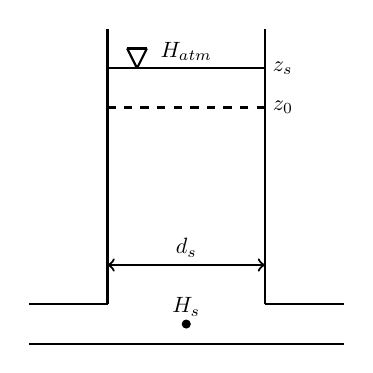
\begin{tikzpicture}[ scale=1, every node/.style={scale=0.8},] 
% Pipe
\draw[thick] (2,0) -- (-2,0);
\draw[thick] (1,0.5) -- (2,0.5);
\draw[thick] (-1,0.5) -- (-2,0.5);
% Sides
\draw[thick] (1,0.5) -- (1,4);
\draw[thick] (-1,0.5) -- (-1,4);
% Water levels
\draw[thick, dashed] (1,3) -- (-1,3);
\draw[thick] (1,3.5) -- (-1,3.5);


% Annotations
\node[anchor=west] at (1,3.5) {$z_s$};
\node[anchor=west] at (1,3) {$z_0$};
\node[anchor=south] at (0,1) {$d_s$};
\draw[thick, <->] (1,1) -- (-1,1);

% Node labels
\draw[fill=black] (0,0.25) circle (0.05cm);
\node[anchor=south] at (0,0.25) {$H_s$};
%\draw[fill=black] (0,3.5) circle (0.05cm);
\node[anchor=south] at (0,3.5) {$H_{\text{atm}}$};
% Free surface symbol
\draw[thick] (-0.5,3.75) -- (-0.75,3.75);
\draw[thick] (-0.5,3.75) -- (-0.625,3.5);
\draw[thick] (-0.75,3.75) -- (-0.625,3.5);
\end{tikzpicture} 
\caption{A surge tank boundary at node $s$ with an a fluid level $z_s$, an initial fluid level $z_0$ and tank diameter $d_s$.}
\label{fig:surge_tank_diagram}
\end{figure}

Suppose that a surge tank is placed in the network at node $s$, at this node we have the continuity equation
\begin{align}
\left( \mathbf{K}^T \right)_s \mathbf{Q} + D_{s,s} \pardiv{}{H_s}{t} = C_s,
\end{align}
where $\left( \mathbf{K}^T \right)_s$ indicates the $s$th row of the matrix $\mathbf{K}^T$ and $D_{s,s}$ indicates the element of the matrix $D$ at row $s$ and column $s$. The flow which leaves the node and fills the surge tank may be modelled by choosing an appropriate expression for the consumption term $C_s$. 

The nodal head $H_s$ is equal to the head due to atmospheric pressure plus the fluid column height i.e.
\begin{align}
H_s = H_{\text{atm}} + z_s.
\end{align} 
The rate at which fluid flows into the surge tank is
\begin{align*}
A_s \frac{d z_s}{d t},
\end{align*}
where $A_s = \pi d_s^2 / 4$ is the cross-sectional area of the tank. If we assume that the fluid in the tank moves as a slug then we may say that
 \begin{align*}
A_s \frac{d z_s}{d t} = A_s \pardiv{}{z_s}{t} = A_s \pardiv{}{H_s}{t}.
\end{align*}
Therefore, since flow into the tank is equal to flow out of the node $(C_s < 0)$, we may rewrite the continuity equation as
\begin{align*}
\left( \mathbf{K}^T \right)_s \mathbf{Q} + D_{s,s} \pardiv{}{H_s}{t} = - A_s \pardiv{}{H_s}{t}.
\end{align*}
Splitting into a known part and correction at the next time step the continuity equation, at node $s$, is given by
\begin{align}\label{discrete_transient_continuity_eqn_surge}
\theta \left( \mathbf{K}^T \right)_s \mathbf{Q}^{n+1,c} + \frac{(D_{s,s} + A_s)}{\Delta t} H_s^{n+1,c} = - \left( \mathbf{K}^T \right)_s \bar{\mathbf{Q}} - \frac{(D_{s,s} + A_s)}{\Delta t} \left( H_s^{n+1,g} - H_s^{n} \right).
\end{align}
The equation \eqref{discrete_transient_continuity_eqn_surge} then substitutes the $s$th row of the system of governing equations \eqref{discrete_transient_system}. It may be observed that by adding the surge tank we are effectively modifying the coefficient $D_{s,s}$ such that $D_{s,s} \rightarrow D_{s,s} + A_s$ thereby reducing the rate at which $H_s$ changes with time for a given set of flow rates through the edges connected to node $s$. 


\subsection{Components}

Components other than pipes may be specified in equation \eqref{discrete_momentum_eqn}. For a general component, of the form shown in figure \ref{fig:general_component}, a relationship between the nodal heads and the pipe flow rate must be specified. 

\begin{figure}
\centering
\begin{tikzpicture}[scale=1, every node/.style={scale=0.8}] 
%\draw[step=1cm,color=gray] (3,0) grid (7,3);
\node[anchor=north] at (3,-0.08) {$H_i$};
\draw[fill=black] (3,0) circle (0.05cm);
\node[anchor=south] at (5,0.08) {$Q_j$};
\draw[thick] (5,0) node[cross=4pt] {};
\node[anchor=north] at (7,-0.08) {$H_k$};
\draw[fill=black] (7,0) circle (0.05cm);
\draw[thick] (3,0) -- (7,0);
\end{tikzpicture} 
\caption{General component $j$ with an average flow rate $Q_j$ and nodal heads $H_i$ and $H_k$.}
\label{fig:general_component}
\end{figure}

% Transient components

%{\color{red}

\subsubsection{Reservoir}

For example a reservoir with an entrance loss 
\begin{align}
h_e = \frac{C_e Q^2}{2 g A^2},
\end{align}
where $C_e$ is the entrance loss coefficient, has resistance term
\begin{align}\label{reservoir_resistance}
R_j =& \frac{(C_e)_j Q_j^2}{2 g A_j^2} \\
\approx & \frac{(C_e)_j }{2 g A_j^2} \left[ \bar{Q}_j^2 + 2 \theta \bar{Q}_j Q_j^{n+1,c}  \right],
\end{align}
where $\bar{Q} = \theta Q_j^{n+1,g} + (1-\theta) Q_j^n$. So if the reservoir boundary is located at node $i$ then we replace the $i$-th contnuity equation with 
\begin{align}
\theta H_i^{n+1,c} = H_{res} - \bar{H}_i
\end{align}
and replace the resistance term in the momentum equation \eqref{discrete_momentum_eqn} with \eqref{reservoir_resistance} and set $L_j = 0$ in $\mathbf{B}$.

}

\subsubsection{Valves}

Transient flows in pipe networks may be caused by the closing and opening of valves. In order to describe the transient behaviour of a valves we must define the valve open ratio $\tau(t)$ as a function of time. The valve open percentage is then used to determine the loss coefficient $k$ in the valve resistance equation \eqref{valve_resistance}.

\paragraph{Closing}
 
 The function $\tau(t)$, as shown in figure \ref{fig:valve_closing}, for a valve closure is given by 
\begin{align}\label{valve_closure_function}
\tau(t) = 
\begin{cases} 
\tau_{steady}, &\text{if} \hspace{0.5cm} t \leq t_e \\
\tau_{steady} \left( 1 - \frac{t-t_e}{t_c} \right)^m, &\text{if} \hspace{0.5cm} t_e \leq t \leq t_e + t_c \\
0, &\text{if} \hspace{0.5cm} t \geq t_e + t_c, 
\end{cases}
\end{align} 
where $t_e$ is the event time, $t_c$ is the time taken for the valve to close, $\tau_{steady}$ is the steady state valve open percentage. The exponent $m > 0$ modifies the shape of the closure profile with $m=1$ corresponding to a linear profile. 
 
\begin{figure}
\centering
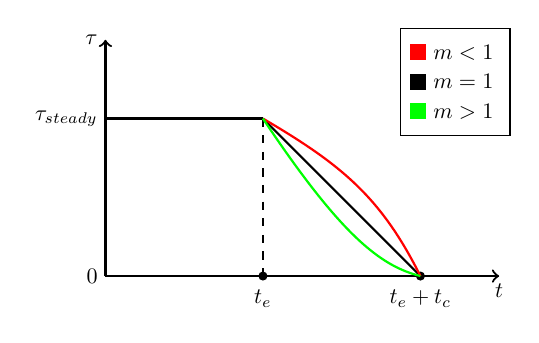
\begin{tikzpicture}[
	scale=1, 
	every node/.style={scale=0.8},
	greennode/.style={shape=rectangle, fill=green, draw=green, minimum size =0.01cm},
	rednode/.style={shape=rectangle, fill=red, draw=red, minimum size =0.01cm},
	blacknode/.style={shape=rectangle, fill=black, draw=black, minimum size =0.01cm},
] 
\draw[thick, ->] (0,0) -- (0,3);
\node[anchor=east] at (0,3) {$\tau$};
\draw[thick, ->] (0,0) -- (5,0);
\node[anchor=north] at (5,0) {$t$};
\node[anchor=north] at (2,-0.08) {$t_e$};
\draw[fill=black] (2,0) circle (0.05cm);
\node[anchor=north] at (4,-0.08) {$t_e + t_c$};
\draw[fill=black] (4,0) circle (0.05cm);
\node[anchor=east] at (0,2) {$\tau_{steady}$};
\draw[thick] (0,2) -- (2,2);
\draw[thick] (2,2) -- (4,0);
\draw[thick, dashed] (2,2) -- (2,0);
\node[anchor=east] at (0,0) {$0$};
\draw[thick, red] (2,2) .. controls (3,1.414) and (3.5,1) .. (4,0);
\draw[thick, green] (2,2) .. controls (3,0.5) and (3.5,0.125) .. (4,0);

\matrix [draw,below left] at (current bounding box.north east) {
  \node [rednode,label=right: {$m < 1$}] {}; \\
  \node [blacknode,label=right: {$m = 1$}] {}; \\
  \node [greennode,label=right: {$m > 1$}] {}; \\
};
\end{tikzpicture} 
\caption{Valve closure. The open ratio $\tau(t)$ goes from $\tau_{steady}$ at time $t_e$ to zero at time $t_e + t_c$, where $t_c$ is the time taken for the valve to close. The exponent $m$ modifies the closure profile, as shown by the red and green curves.}
\label{fig:valve_closing}
\end{figure}

\paragraph{Opening}

The function $\tau(t)$, as shown in figure \ref{fig:valve_opening}, for a valve opening is given by 
\begin{align}\label{valve_opening_function}
\tau(t) = 
\begin{cases} 
\tau_{steady}, &\text{if} \hspace{0.5cm} t \leq t_e \\
\tau_{steady} + \left( 1 - \tau_{steady} \right) \left( \frac{t-t_e}{t_c} \right)^m, &\text{if} \hspace{0.5cm} t_e \leq t \leq t_e + t_c \\
1, &\text{if} \hspace{0.5cm} t \geq t_e + t_c, 
\end{cases}
\end{align} 
where $t_e$ is the event time, $t_c$ is the time taken for the valve to close, $\tau_{steady}$ is the steady state valve open percentage. The exponent $m > 0$ modifies the shape of the opening profile with $m=1$ corresponding to a linear profile. 

\begin{figure}
\centering
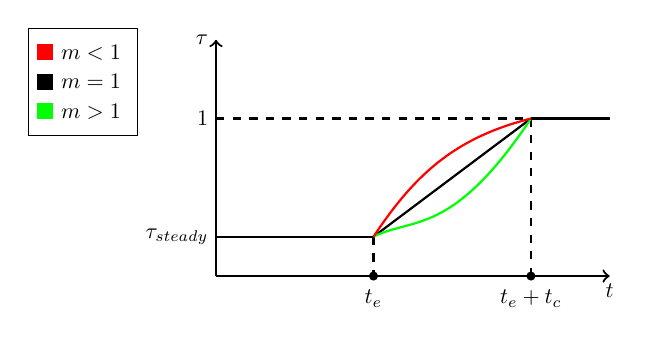
\begin{tikzpicture}[
	scale=1, 
	every node/.style={scale=0.8},
	greennode/.style={shape=rectangle, fill=green, draw=green, minimum size =0.01cm},
	rednode/.style={shape=rectangle, fill=red, draw=red, minimum size =0.01cm},
	blacknode/.style={shape=rectangle, fill=black, draw=black, minimum size =0.01cm},
] 
\draw[thick, ->] (0,0) -- (0,3);
\node[anchor=east] at (0,3) {$\tau$};
\draw[thick, ->] (0,0) -- (5,0);
\node[anchor=north] at (5,0) {$t$};
\node[anchor=north] at (2,-0.08) {$t_e$};
\draw[fill=black] (2,0) circle (0.05cm);
\node[anchor=north] at (4,-0.08) {$t_e + t_c$};
\draw[fill=black] (4,0) circle (0.05cm);
\node[anchor=east] at (0,0.5) {$\tau_{steady}$};
\draw[thick] (0,0.5) -- (2,0.5);
\draw[thick] (2,0.5) -- (4,2);
\draw[thick, dashed] (2,0.5) -- (2,0);
\draw[thick, dashed] (4,0) -- (4,2);
\draw[thick, dashed] (0,2) -- (4,2);
\node[anchor=east] at (0,2) {$1$};
\draw[thick, green] (2,0.5) .. controls (2.5,0.75) and (3,0.5) .. (4,2);
\draw[thick, red] (2,0.5) .. controls (2.5,1.25) and (3,1.75) .. (4,2);
\draw[thick] (4,2) -- (5,2);


\matrix [draw,below left] at (current bounding box.north west) {
	\node [rednode,label=right: {$m < 1$}] {}; \\
	\node [blacknode,label=right: {$m = 1$}] {}; \\
	\node [greennode,label=right: {$m > 1$}] {}; \\
};
\end{tikzpicture} 
\caption{Valve opening. The open ratio $\tau(t)$ goes from $\tau_{steady}$ at time $t_e$ to one at time $t_e + t_c$, where $t_c$ is the time taken for the valve to close. The exponent $m$ modifies the closure profile, as shown by the red and green curves.}
\label{fig:valve_opening}
\end{figure}

\subsubsection{Pumps}

The starting and stopping of pumps are a significant cause of transient flows in pumping systems. Starting of a pump is usually controlled by keeping the discharge valve close until the pump reaches the rated speed and then slowly opening the valve. However sometimes pumps are started without using valves by controlling the speed electronically. Similarly pump shutdown may be assisted by valve closure or by external control. Another common source of pump transients is power failure, in this situation the speed of the pump is no longer controlled and is instead determined by the torque on the pump and the flow conditions.  

\paragraph{Shutdown}

The simplest way to shutdown a pump in a controlled manner is a reduction of the rotational speed, at a specified event time $t_e$, to zero at time $t_e + t_c$, where $t_c$ is stopping time. The rotational speed $N$ as a function of time $t$, as shown in figure \ref{fig:pump_shutdown}, is defined by the piecewise function
\begin{align}\label{pump_shutdown_function}
N(t) = 
\begin{cases} 
N_{steady}, &\text{if} \hspace{0.5cm} t \leq t_e \\
N_{steady} \left( 1 - \frac{t-t_e}{t_c} \right)^m, &\text{if} \hspace{0.5cm} t_e \leq t \leq t_e + t_c \\
0, &\text{if} \hspace{0.5cm} t \geq t_e + t_c. 
\end{cases}
\end{align}
The exponent $m > 0$ modifies the shape of the closure profile with $m=1$ corresponding to a linear profile. Changing the rotational speed alters both $n$ and $\theta$ in the pump resistance equation \eqref{pump_resistance} so that the resistance varies with time too. 

\begin{figure}
\centering
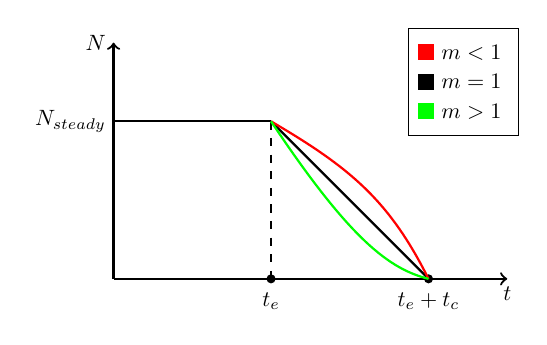
\begin{tikzpicture}[
	scale=1, 
	every node/.style={scale=0.8},
	greennode/.style={shape=rectangle, fill=green, draw=green, minimum size =0.01cm},
	rednode/.style={shape=rectangle, fill=red, draw=red, minimum size =0.01cm},
	blacknode/.style={shape=rectangle, fill=black, draw=black, minimum size =0.01cm},
] 
\draw[thick, ->] (0,0) -- (0,3);
\node[anchor=east] at (0,3) {$N$};
\draw[thick, ->] (0,0) -- (5,0);
\node[anchor=north] at (5,0) {$t$};
\node[anchor=north] at (2,-0.08) {$t_e$};
\draw[fill=black] (2,0) circle (0.05cm);
\node[anchor=north] at (4,-0.08) {$t_e + t_c$};
\draw[fill=black] (4,0) circle (0.05cm);
\node[anchor=east] at (0,2) {$N_{steady}$};
\draw[thick] (0,2) -- (2,2);
\draw[thick] (2,2) -- (4,0);
\draw[thick, dashed] (2,2) -- (2,0);
\draw[thick, red] (2,2) .. controls (3,1.414) and (3.5,1) .. (4,0);
\draw[thick, green] (2,2) .. controls (3,0.5) and (3.5,0.125) .. (4,0);

\matrix [draw,below left] at (current bounding box.north east) {
  \node [rednode,label=right: {$m < 1$}] {}; \\
  \node [blacknode,label=right: {$m = 1$}] {}; \\
  \node [greennode,label=right: {$m > 1$}] {}; \\
};
\end{tikzpicture} 
\caption{Pump shutdown. The rotational speed $N(t)$ goes from $N_{steady}$ at time $t_e$ to zero at time $t_e + t_c$, where $t_c$ is the time taken for the pump to stop. The exponent $m$ modifies the closure profile, as shown by the red and green curves.}
\label{fig:pump_shutdown}
\end{figure}

\paragraph{Startup}

The time varying function describing the startup of a pump, as shown in figure \ref{fig:pump_startup}, is very similar to the function describing a shutdown and is given by 

\begin{align}\label{pump_startup_function}
N(t) = 
\begin{cases} 
0, &\text{if} \hspace{0.5cm} t \leq t_e \\
N_{\infty} \left( \frac{t-t_e}{t_s} \right)^m, &\text{if} \hspace{0.5cm} t_e \leq t \leq t_e + t_s \\
N_{\infty}, &\text{if} \hspace{0.5cm} t \geq t_e + t_s, 
\end{cases}
\end{align}
where again $t_e$ is the event time, $t_s$ is startup time and $N_{\infty}$ is the pump speed once the startup procedure has been completed. The exponent $m > 0$ modifies the shape of the closure profile with $m=1$ corresponding to a linear profile. 


\begin{figure}
\centering
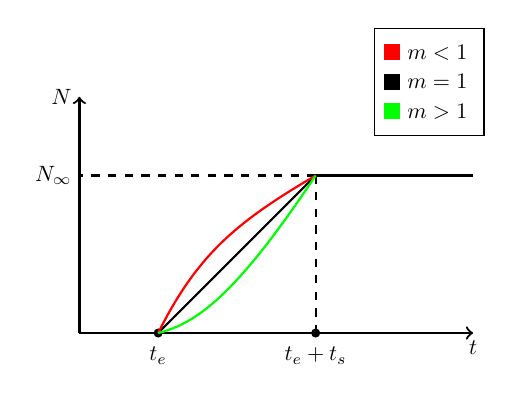
\begin{tikzpicture}[
	scale=1, 
	every node/.style={scale=0.8},
	greennode/.style={shape=rectangle, fill=green, draw=green, minimum size =0.01cm},
	rednode/.style={shape=rectangle, fill=red, draw=red, minimum size =0.01cm},
	blacknode/.style={shape=rectangle, fill=black, draw=black, minimum size =0.01cm},
] 
\draw[thick, ->] (0,0) -- (0,3);
\node[anchor=east] at (0,3) {$N$};
\draw[thick, ->] (0,0) -- (5,0);
\node[anchor=north] at (5,0) {$t$};
\node[anchor=north] at (1,-0.08) {$t_e$};
\draw[fill=black] (1,0) circle (0.05cm);
\node[anchor=north] at (3,-0.08) {$t_e + t_s$};
\draw[fill=black] (3,0) circle (0.05cm);
\node[anchor=east] at (0,2) {$N_{\infty}$};

\draw[thick] (3,2) -- (5,2);
\draw[thick] (1,0) -- (3,2);
\draw[thick, dashed] (3,2) -- (3,0);
\draw[thick, dashed] (3,2) -- (0,2);
\draw[thick, red] (1,0) .. controls (1.5,1) and (2,1.414)  .. (3,2);
\draw[thick, green] (1,0) .. controls (1.5,0.125) and (2,0.5) .. (3,2);

\matrix [draw,left] at (current bounding box.north east) {
  \node [rednode,label=right: {$m < 1$}] {}; \\
  \node [blacknode,label=right: {$m = 1$}] {}; \\
  \node [greennode,label=right: {$m > 1$}] {}; \\
};
\end{tikzpicture} 
\caption{Pump startup. The rotational speed $N(t)$ goes from zero at time $t_e$ to $N_{\infty}$ at time $t_e + t_s$, where $t_s$ is the time taken for the pump to startup. The exponent $m$ modifies the closure profile, as shown by the red and green curves.}
\label{fig:pump_startup}
\end{figure}

% \paragraph{General speed variation (piecewise linear)}

% \paragraph{Power failure}

\subsubsection{Relief valves}

\paragraph{Pressure relief valves}

\paragraph{Safety valves}

\subsubsection{Check / Non-return valves}

A check or non-return valve is a valve that allows fluid to flow through it in one direction only. \ 
The resistance of a check valve has the same form as for a standard valve, see equation \ 
\eqref{valve_resistance}, however the inverse loss coefficient $k_j^{-1}$ is given by
\begin{align}
    \boxed{ 
        k_j^{-1} = 
        \begin{cases}
            0, & \text{if } \Delta H_j \leq 0, \\
            k_0^{-1}, & \text{if } \Delta H_j > 0.
        \end{cases}
    }
\end{align}
This means that the check valve is open when the pressure difference across it is positive and \ 
closed when the pressure difference is negative. The value $k_0$ is the loss coefficient of the \ 
valve when it is fully open. For steady flow, the check valve is considered to be open \ 
$(\tau = 1)$, so the inverse loss coefficient is $k_0^{-1}$. 
